\subsubsection{10}

\zadatak
Re{\sv}i nejedna{\cv}inu
$$
\log_5 x \ge \frac12 \log_5(3x-2).
$$

\resenje
Da bi logaritam bio definisan, vidimo da mora biti
$$
3x-2>0\sledi x>\frac23.
$$
Ako nejedna{\cv}inu pomo{\zv}imo sa 2 , dobijamo
\begin{align*}
    2\log_5 x   &\ge \log_5(3x-2)\\
    \log_5 x^2  &\ge \log_5(3x-2)\\
    x^2 &\ge 3x-2\\
    x^2 -3x + 2 &\ge 0.
\end{align*}
Kvadratna jedna{\cv}ina ima re{\sv}e{\nj}a $x_1=1$ i $x_2=2$,
pa je re{\sv}e{\nj}e nejedna{\cv}ine
$$
x\in\ram{\left( \frac23, 1 \right] \cup  [2, \infty )}.
$$
%\vskip-18pt
%$$
%\slika{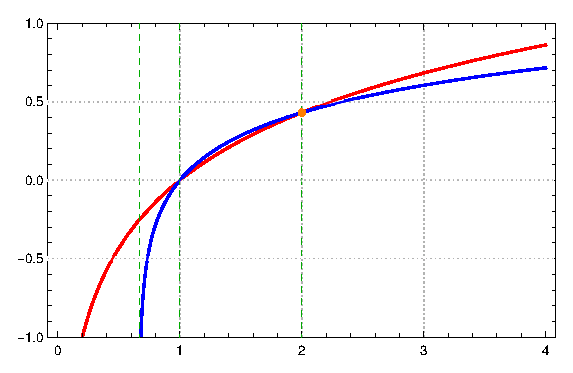
\includegraphics[width=100\mm]{eps/10.eps}}{$y=\log_5 x - \frac12 \log_5(3x-2)$}
%$$

